%% Template for SDP report, adapted from mlp_cw2_template, 2018. 

%% Based on  LaTeX template for ICML 2017 - example_paper.tex at 
%%  https://2017.icml.cc/Conferences/2017/StyleAuthorInstructions

\documentclass{article}
\usepackage[T1]{fontenc}
\usepackage{amssymb,amsmath}
\usepackage{txfonts}
\usepackage{microtype}
\usepackage{xspace}
\xspaceaddexceptions{\%}

% Lists with less spacing between items
\usepackage{paralist}

% For figures
\usepackage{graphicx}
\usepackage{subfig} 

% For citations
\usepackage{natbib}

% For algorithms
\usepackage{algorithm}
\usepackage{algorithmic}

% the hyperref package is used to produce hyperlinks in the
% resulting PDF.  If this breaks your system, please commend out the
% following usepackage line and replace \usepackage{mlp2017} with
% \usepackage[nohyperref]{mlp2017} below.
\usepackage{hyperref}
\usepackage{url}
\urlstyle{same}

% Packages hyperref and algorithmic misbehave sometimes.  We can fix
% this with the following command.
\newcommand{\theHalgorithm}{\arabic{algorithm}}


% Set up MLP coursework style (based on ICML style)
\usepackage{mlp2018}
\mlptitlerunning{SDP Demo \demoNumber  Group (\groupNumber)}
\bibliographystyle{icml2017}


\DeclareMathOperator{\softmax}{softmax}
\DeclareMathOperator{\sigmoid}{sigmoid}
\DeclareMathOperator{\sgn}{sgn}
\DeclareMathOperator{\relu}{relu}
\DeclareMathOperator{\lrelu}{lrelu}
\DeclareMathOperator{\elu}{elu}
\DeclareMathOperator{\selu}{selu}
\DeclareMathOperator{\maxout}{maxout}







%% You probably do not need to change anything above this comment

%% REPLACE the details in the following commands with your details
\setGroupNumber{18}
\setGroupName{Opticane}
\setProductName{Opticane}
\setDemoNumber{4}
\setLogoFileName{figs/opticane-logo.png}

\begin{document} 

\makeSDPTitle{Demo}

% Previous MLP Style Title Layout working. 
% \twocolumn[
    % \mlptitle{\productName: SDP Demo \demoNumber}
    % \centerline{Group \groupNumber: \groupName}
% ]

\begin{abstract} 
Opticane is a self-contained cane for the visually impaired that translates a user's surroundings to haptic feedback in the handle.

For the final demo, we've completed our hardware, software, prototype, website, and user guide. We have completed the integration of our purchased LIDAR, servo motor, and vibration motor communication, 3D printed Opticane's handle and fitted our hardware components inside of it, wrote content for our website, and completed our user guide.    
\end{abstract} 

\section{Project plan update} 

After receiving our last demo's feedback, the goals that we planned to achieve for this demo were:
\begin{itemize}
    \item Hardware 4.1: Establish LIDAR data to Vibration Motors Communication (achieved)
    \item Hardware 4.2: 3D Print Prototype with Garry (achieved)
    \item Software 4.1: Complete Written Content for Website (achieved)
    \item Software 4.3: Implement Technical Complexities in Simulation (achieved)
    \item Research 4.1: Conduct Quantitative and Qualitative Analysis (achieved)
    \item Research 4.2: Continue Ethics Report (achieved)
    \item Research 4.3: Continue Literature Review (achieved)
    \item Presentation 4.1: Create Graphics for Demo (achieved)
    \item Presentation 4.2: 3D Model Alternative Cane Grips (achieved)
    \item Presentation 4.3: Complete User Guide (achieved)
    \item Presentation 4.4: Finish Pitch Video (achieved)
    \item Presentation 4.5: Complete Poster (achieved)
    
\end{itemize}

Our group was able to achieve all of these goals and in doing so, finalize all of our hardware implementation, create a prototype, complete our website, and write our user guide. To meet these goals, we utilized Trello, Github, and Microsoft Teams with detailed tickets, thoroughly reviewed code pull requests, and weekly scrum meetings.

To promote parallel working, we split our group into teams similarly to the last demo. This time, Lewis, Yuanting, and Austin worked on hardware; Samuel and Ioana worked on software; Iman, Lewis, and Ioana worked on research; and everyone worked on presentation.

Working on these separate parts, we estimate that we've spent about 200 hours total on demo 4. Compared to demo 3, in demo 4, we've focused a lot more time on the final presentation of our website, video, and user guide. In addition, we've tried to come up with more numerical results for quantitative analysis from literature. The tiem breakdown is covered in figure \ref{fig:time-fig} while the task breakdown is covered in figure \ref{fig:tickets}.

\begin{figure}[tb]
\vskip 5mm
\begin{center}
\centerline{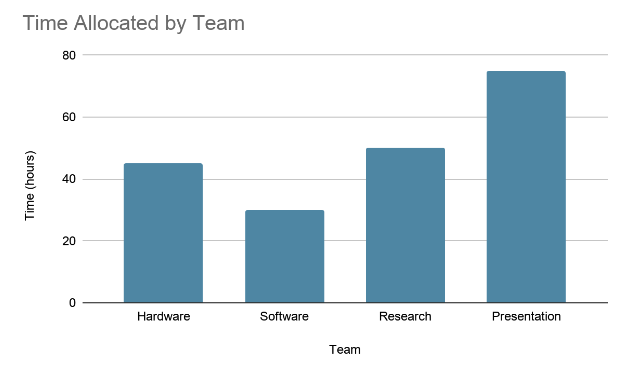
\includegraphics[width=\columnwidth]{figs/time-breakdown}}
\caption{Time Breakdown}
\label{fig:time-fig}
\end{center}
\vskip -5mm
\end{figure} 

Moving forward, we would like to finalize our website, make tweaks to our video, and set up our gather.town space in preparation for the industry day.

\section{Technical details}

\subsection{Prototype}

For the final demo, we've produced an initial prototype of Opticane. Our prototype consists of a 3D printed cane handle along with the hardware components placed inside to demonstrate our most basic functionality: object detection.

On the hardware side, we've completed the communications between our custom rotating LIDAR and disc vibration motors using a multiplexer. While implementing this, we found a few difficulties in the documentation of the LIDAR with which bits contained the relevant distance information and our initial multiplexer set up had one i2c multiplexed port not functioning as intended. After overcoming these challenges, however, we've been able to successfully have the vibration motors react to the objects detected by the LIDAR.

For the housing of the hardware, we've 3D printed our cane handle, raspberry pi case, battery case, and LIDAR case to hold all of our components together and have a working prototype that can perform object detection. The 3D printing process had a few challenges in that a few of our casings were modeled to have the lid exactly fit its case, but in-person this wasn't practical and we had to give the lid and case a bit of breathing room so that the fitting process of the lid on the case was much smoother.

\subsection{3D Model}

Building on our original 3D model, we've attached our LIDAR casing below the base of the handle to show the arrangement of all of our parts in-person. We have also added an LED and microphone mesh to account for the low light LED and voice recognition we implemented in the last demo. In addition, to make our haptic feedback more intuitive, we've added small bumps to each vibration motor indicating the direction that the motor corresponds to. Finally, we had to model a custom part to attach the LIDAR to the servo horn.

In addition to our original 3D model which models a handle grip for an overhand grasp, the most popular grip type, we've made two additional models that account for the pencil grip and the angled walking cane grip. These additional handles allow for Opticane to serve a larger audience of users who have different preferences in how they hold their canes.

In terms of size, the prototype suits someone who is size 11 or extra large for work gloves. According to work glove size scales, we plan on supporting sizes ranging from 7 to 11, covering small, medium, large, and extra large as the optional handle sizes for customers. \cite{3glove}

We've also imported our models into Blender to create photorealistic renders and animations of our handles for our website and pitch video. A rendered image can be found in figure \ref{fig:render}.

\subsection{Simulation}

For our simulation, we've integrated the technical complexities of our last demo into our current simulation that consists of human controllers that swing white canes from side to side with a working LIDAR. This includes our haptic navigation, voice recognition, and battery indication.

Using human PROTO controllers, we can specify joint angles as well as destination points for the pedestrian to walk to. With this, we can have the user pause on keyboard input to wait for a voice command, and when provided, act on it accordingly. When using haptic navigation, the console outputs the feedback that indicates the direction of the destination and then the user walks towards the destination. For battery checking, we use a dummy battery percentage that is communicated to the user with haptic feedback which is modeled in the output console.

\subsection{Presentation}

We have also completed the written content of our website and finished our poster, aiming for a professional and modern graphic and design scheme. The website is one long scrollable page that consists of how our system works, market research, budget, evaluation, and information about our team. We also wrote a short design guide to adhere to for our website and poster.

\subsection{Literature Review}
 
One feature we’d like to introduce into our cane that is not found on other canes is haptic feedback for percentage levels of the battery. While haptic feedback has existed for indicating to a user that the battery level is low, such as the vibration found in old Nokia phones or video game controllers, we wanted to give users  much more detailed information so that they can know exactly how much battery is left and be confident in how long they can use the cane. However the main issue with this is that visually impaired people find the inherent visual medium of percentages hard to comprehend since they do not view information in the same way sighted people do. \cite{7wolchover} There is little literature on how to convert such percentages to a haptic format that blind people can cognitively realise however we believe by extending the features of current haptics in UI we can create a haptic language for representing battery life. In a study by Immersion, most people (78\%) recognise the haptic vibration for an incoming message or alert- the more forceful the haptic the more alerted the user. \cite{8immersion} If we take the logic as more haptic feedback translates to more important information and the less battery life the more we would want to alert the user (i.e the more important the cane’s situation. Therefore if we set all 5 haptic motors to go off to show battery life is very low the  visually impaired user intuitively understands the importance of the situation and we can then decrease the amount of haptics to represent different stages of alertness, i.e.

\begin{itemize}
    \item 5 Motors = user very alerted, battery about to die
    \item 4 Motors = user quite alerted, battery is low
    \item 3 Motors = user alerted, battery on half
    \item 2 Motors = user slighted alerted to level they can ignore, battery close to full
    \item 1 Motor = user alert at a minimum, user can safely ignore, battery is full
\end{itemize}

Unlike our developed Haptic language for battery life, haptic feedback for navigational information is far better researched. An MIT study concluded that through user testing haptic feedback navigation was feasible. \cite{9ertan} In fact the study found that when the array of micrometers vibrated (they would use 8 micrometers in tandem to represent different pole positions relative to the user) the users found the vibrations “soothing”. A further study, looked into representing more complex map information via haptics and showed that such real world information could be represented by Haptics. The study concluded it was “easy for (users) to learn the vibrational patterns for horizontal and vertical lines \dots and for certain diagonal lines” Therefore we have confidence that our navigation system where each motor represents a direction the user can go in will be intuitive and easy-to-use. \cite{10grussenmeyer}
 
This study however also emphasised the importance of a tutorial of the haptic device to allow visually-impaired people to orient themselves to such a haptic language. This is something we would definitely implement in future iterations of the product. It would be a dimple system where the voice recognition command of “tutorial” where the user would feel a vibration and a speaker on the cane would tell the user which direction that vibration represents. The tutorial would also cover the Haptic language of the battery life, based on studies, would be intuitive and could also help users map general numbers to the haptics as well.
 
Finally we looked at the literature on white canes with lights on them. There are current devices on the market which add LEDs to the tips of non-smart white canes to indicate where a user is at night such as the StrideLight The Blind Guide website spoke about how such as product helped give people confidence to walk at night, as the cane indicates to others that they are there. \cite{11henkler} We decided to implement such a feature into our cane, initially settling on a standard LED. However with many studies showing that LED headlights have a tendency to dazzle other drivers on the road  we would also perhaps look into using an LED with a much warmer white, such as the warm colour found on halogen light bulbs. \cite{12marshall} These warmer colours are far less likely to dazzle other pedestrians, keeping our users and others safe.

\section{Evaluation}

\subsection{Quantitative Analysis}

For our final hardware prototype of the cane, we’ve endeavoured to find the smallest and lightest hardware components possible that still allow for the same level of functionality. We have just assumed that the lighter the cane the better without researching what are the optimal and also minimum acceptable cane weights. In a 2013 study, it was found that lighter canes made of carbon fibre (around 113g) did not strain the wrist and upper muscles as much as conventional canes weighing around 252g “results indicated that the newly developed cane reduced the loads on muscles by approximately 50\%”. \cite{13doi} This tells us that for a comfortable final product the actual cane itself should be a newer carbon-fibre model. Additionally it gives us parameters to work with in terms of 252g is the acceptable cane weight so we should select parts for the cane handle to ensure the combined weight of the carbon fibre cane and the handle is less than 252g. Currently our TF Luna Lidar is 5g, the MG90s Servo Motor is 14g, Raspberry Pi Zero is 9g, the RS Pro battery is 21g and we’d estimate the weight of the casing at around 150g. Therefore we’d hope the final product’s weight is around 200g thereby being closer to the optimal weight of a whitecane.
 
One question asked in the last demo’s marking is whether haptic feedback is affected by the cane hitting the ground. This type of question would usually be resolved by in-person user testing however due to that being unavailable, looking to literature can help find an answer. In a 2010 paper by École Polytechnique Fédérale de Lausanne they designed a similar sort of ‘smart cane’ with haptic feedback, albeit the source of the haptic feedback only coming from one motor. \cite{14gallo} The design used an inertia wheel and mentioned a good force for haptic feedback was between 1000 and 4000 milli Newtons. The paper also mentioned that more powerful motors, larger than our coin buzzer motors, may generate too much force that could potentially damage other parts of the handle. Operating at 5V, our mini disc motors will generate a minimum force around 2500mN so even the weakest force can be distinguished from the general haptic of a cane hitting off the ground. \cite{15rsOnline}
 
According to the Benewake TF Luna's Datasheet, we get the highest accuracy when the object is between 0.2m and 8m away from the LiDAR. \cite{19mouser}

\subsection{Interview}

We initially wanted to interview people from Tech Era, an organization that works with disabled people, as they would have more insight on our product. But unfortunately our ethics approval was denied because interviewing the visually impaired through Tech Era was considered too specific of an interview group. We have also reached out to the PR team and co-founders of WeWALK, Kursat Ceylan and Sadik Unlu, a company that develops smart canes, to see if we could interview them for advice on designing smart canes. \cite{2wewalk}

While we weren't able to interview visually impaired individuals or the employees of WeWALK, we have instead interviewed some of our fellow students to get some feedback on our project, sending an approved consent form to each interviewee before we conducted our interview. We understand that our interviewees are not representative of the target audience of Opticane, but they were the only accessible individuals due to SDP research restrictions.

All of our participants agreed that users of the standard white cane would encounter disruptions because the cane would not be able to detect some objects. One participant said, “It happens every day if they are alone. It is likely to happen, walking without a guide dog.” and another participant said, “Yes but not that frequently. Because they are accustomed to that life, but when they are in a new environment it definitely would be a problem.”

The main concerns of our project were how users would be confused about the buzzer placement and how users might get anxious if they are in a crowded place and all the buzzers go off. To combat this, we would like to potentially implement a dampener of the haptic feedback when it is triggered for long periods of time given more time.

There were different opinions about what the minimum battery life should be ranging from 6 hours to 12 hours. Lastly, a common suggestion was to have a portable battery and a way to communicate when the battery needs charging which we would like to implement given more time.

\subsection{Ethics Report}

Speech recognition systems sparked a debate regarding the privacy of the users. Jay Staley mentions a striking story concerning "a warrant from police in Arkansas seeking audio records of a man’s Amazon Echo has sparked an overdue conversation about the privacy implications of 'always-on' recording devices". \cite{17stanley}  “Always-on” recording systems are present more and more in our life, but they need to be treated with more caution. 

"Many devices are programmed to keep their microphones on at all times but only record and transmit audio after hearing a trigger phrase—in the case of the Echo, for example, 'Alexa.'" \cite{17stanley} Any device that is to be activated by voice alone must work this way. However, there are a range of other systems. For example, "Samsung \dots assured the public that its smart televisions (like others) only record and transmit audio after the user presses a button on its remote control." \cite{17stanley}

Nevertheless, there is always the risk that the companies lie about their product, which occurred with Volkswagen, that devices get hacked, or that government agencies might try to order companies to use their products for surveillance.

Because of these ethical concerns and the recommendations proposed by Stanley, we've kept our device offline, only recording the user's voice when a button is pushed and then that recording is deleted afterwards.

In our final product, we are planning on implementing a GPS system. "The Global Positioning System (GPS) is increasingly being adopted by private and public enterprises to track and monitor humans for location-based services (LBS)." \cite{18michael} The greatest concern of GPS tracking is the amount of information that can be deduced from the analysis of a person’s movements. 

Moreover, GPS can be prone to errors. "Dense forest, tall buildings, cloud cover and moisture produce inaccuracies in readings but these are considered negligible when compared to the potential for inaccuracies in resultant information processing." \cite{18michael} In that case, the important question is who is liable for the accuracy of the information. "Software used to store tracking data makes it possible to edit data points in order to create false evidence." \cite{18michael} For example, someone can be accused of a crime they did not commit. That’s why it is important to have clear regulations regarding the use of GPS. 

Finally, "the innovative nature of the technology should not be a cause to excuse it from the same 'judicial or procedural constraints which limit the extent to which traditional surveillance technologies are permitted to infringe privacy'" and it is important to have the implementers of GPS systems think about the moral implications of their work. \cite{18michael}

That’s why, the only GPS data we would store would be related to the saved marker locations used for haptic navigation. If an outsider were to somehow gain access to the system, that data would also be the only data accessible because we don't store anything else and our system is offline.

\section{Budget}

In terms of budget, for demo 4, we haven't made any additional purchases for components. This table gives a breakdown of any costs incurred while developing prototypes for the Opticane. Many items such as the HS322 Servo Motor and Raspberry Pi 2 Model B were used as Proof-of-Concept hardware, to be eventually replaced by smaller, more cost efficient versions that will be used in the final commercial product. Also the miniature light bulbs were used as proof of concept haptic feedback for an earlier demo; showing how we could translate LiDAR data to haptic feedback information. A further breakdown can be found in figure \ref{fig:budget-fig}.

We also met with Benedetta to discuss ethical concerns of Opticane as well as to review our interview process and Ryan Bowler to discuss aspects of our user guide.

For technician time, we've mainly been working with Garry to 3D print, assemble, and test our prototype which has taken about 2 hours of active supervision.

\section{Video}

\href{https://uoe-my.sharepoint.com/:v:/g/personal/s1870157_ed_ac_uk/EVPEufrB3jRPn-EKBOmDpfsBlt8M4U8_-mNtX9ykO4Ew1A?e=GiO15D}{video}

%% Include any references in a bibliography
\bibliography{refs}

\begin{figure}[tb]
\vskip 5mm
\begin{center}
\centerline{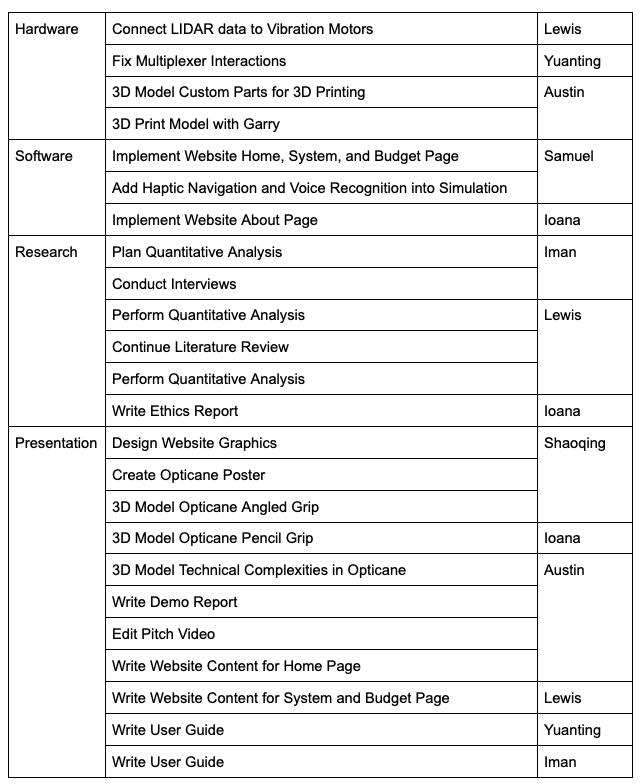
\includegraphics[width=\columnwidth]{figs/task-breakdown}}
\caption{Task Breakdown}
\label{fig:tickets}
\end{center}
\vskip -5mm
\end{figure}

\begin{figure}[tb]
\vskip 5mm
\begin{center}
\centerline{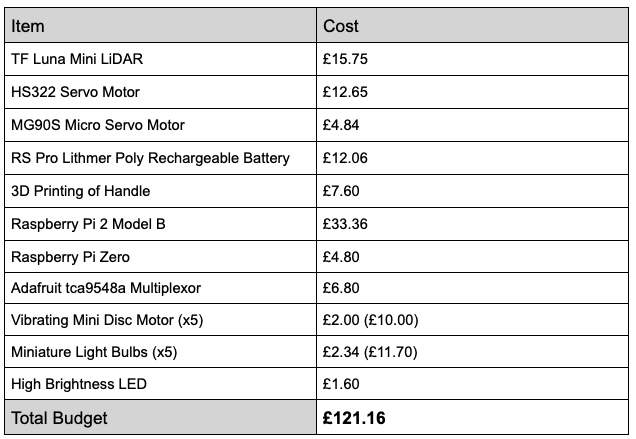
\includegraphics[width=\columnwidth]{figs/budget-breakdown}}
\caption{Budget Breakdown}
\label{fig:budget-fig}
\end{center}
\vskip -5mm
\end{figure}

\begin{figure}[tb]
\vskip 5mm
\begin{center}
\centerline{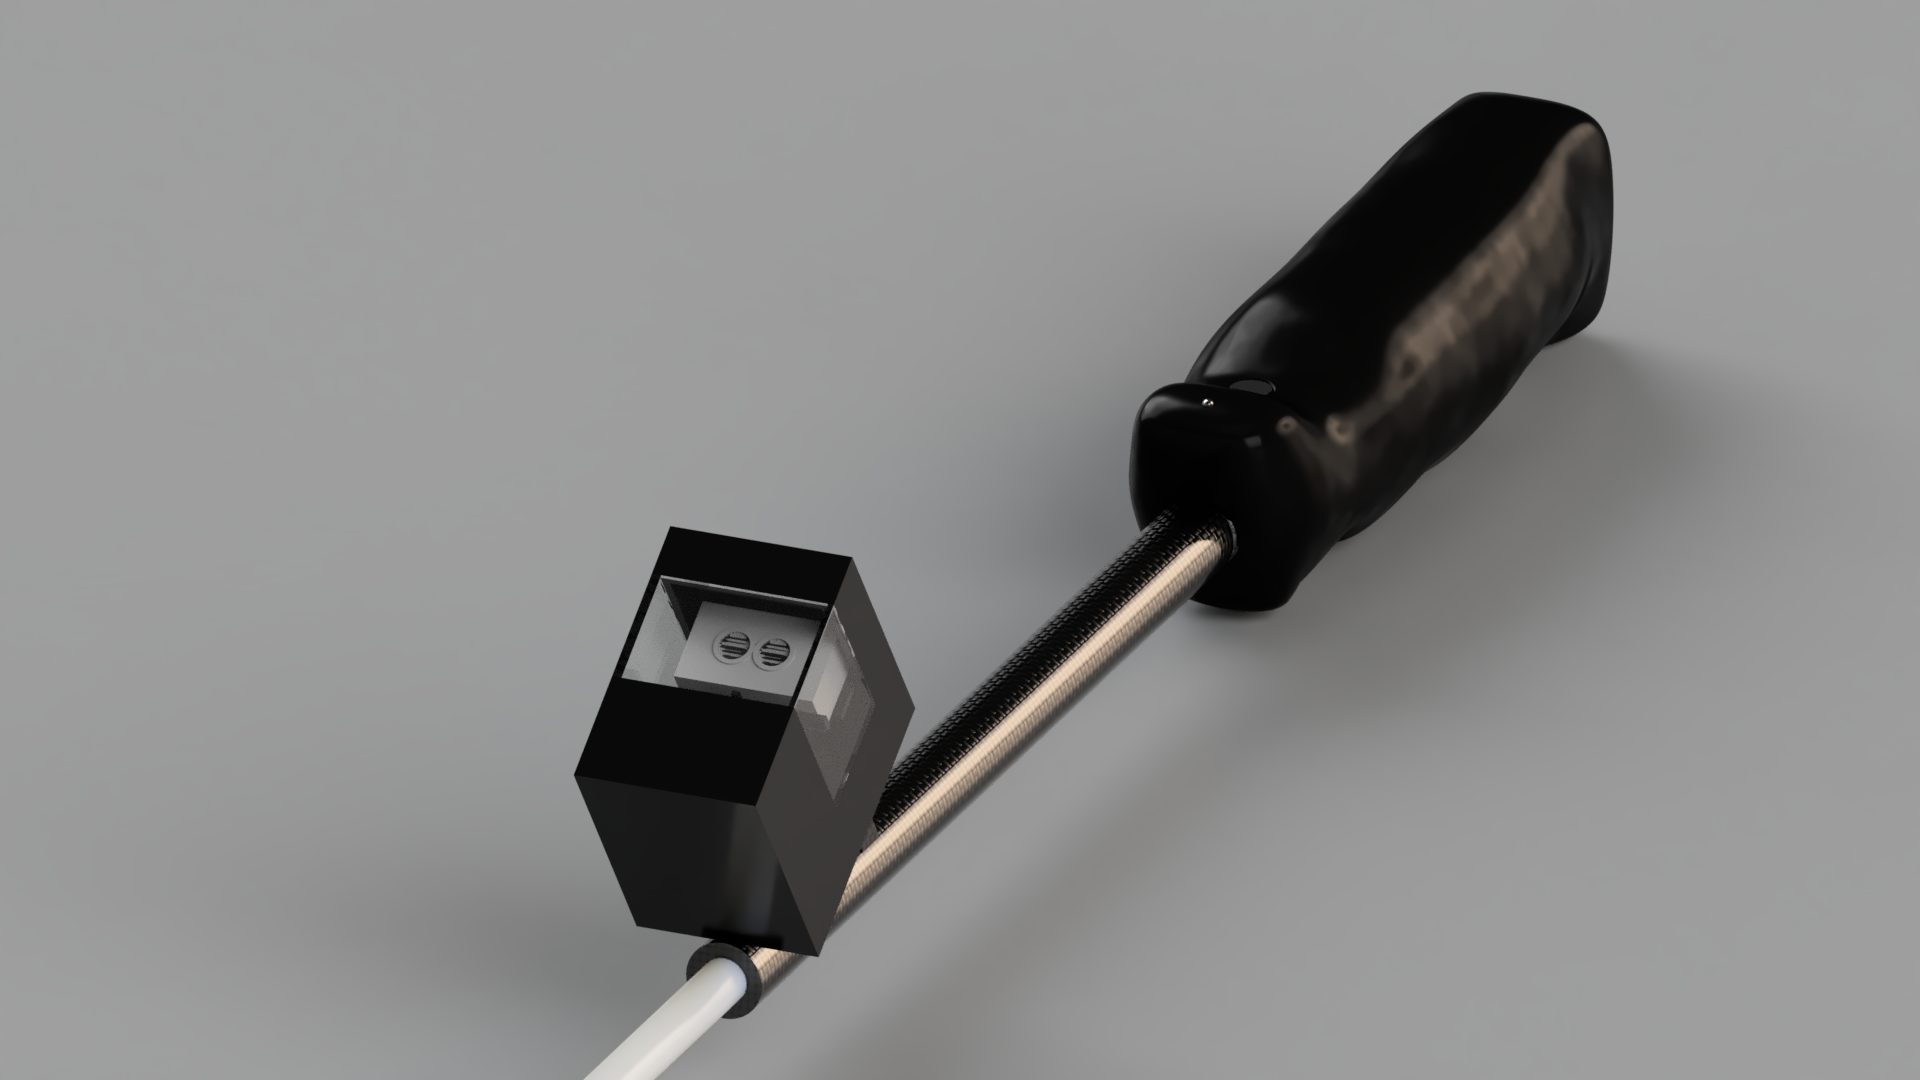
\includegraphics[width=\columnwidth]{figs/handle-render}}
\caption{Opticane Render}
\label{fig:render}
\end{center}
\vskip -5mm
\end{figure}

\end{document} 

